\documentclass[letterpaper,10pt]{book}
% Change to 10 pt
\usepackage{pdfpages}
\usepackage{morewrites}			% to counteract the no write space problem
\setcounter{tocdepth}{6}

\usepackage[framemethod=TikZ]{mdframed}

\usepackage{fancyhdr}

\usepackage{paralist}
\usepackage{amsmath}
\usepackage{amsfonts}
\usepackage{amssymb}
\usepackage{graphicx}

\usepackage{datetime}
%\usepackage{ulem}

%\usepackage[nottoc]{toobibind}

\usepackage[inline]{enumitem}

% Outer margin at 2.50 is exacty correct to fit the ``corruption alert'' tables
\usepackage[inner=1.0in, outer=2.50in, top=2.54cm,bottom=2.54cm, marginparwidth=2.25in]{geometry}

\usepackage{marginnote}
\usepackage{longtable}
\usepackage{booktabs}
\usepackage{xcolor}

\usepackage{soul}

%%%%%%%%%%%%
\definecolor{ForestGreen}{rgb}{0.00,0.29,0.098}
%%%%%%%%%%%%

\usepackage{marginnote}

\usepackage{imakeidx} 
\usepackage[
	backref=true,
	style=numeric,
%	citestyle=numeric,
	backend=bibtex
	]{biblatex}
\usepackage[driverfallback=hypertex,colorlinks=True]{hyperref}
\usepackage{cleveref}

\makeindex[name=scripture,columnsep=20pt, columnseprule=True,columns=3, title=Scripture References]
\makeindex[name=speaker,columnsep=20pt, columnseprule=True,,columns=2, title=Sermon Creator]
\makeindex[name=series,columnsep=20pt, columnseprule=True,,columns=2, title=Sermon Series]
\makeindex[name=date,columnsep=20pt, columnseprule=True,columns=2, title=Sermon Date]
\makeindex[name=event,columnsep=20pt, columnseprule=True,columns=2, title=Event]
\makeindex[name=topic,columnsep=20pt, columnseprule=True,columns=2, title=Topic]
\makeindex[name=AWIP,columnsep=20pt, columnseprule=True,columns=3, title=All Words in Passage]
\makeindex[name=NWIV,columnsep=20pt, columnseprule=True,columns=3, title=Number of Words in Verse]
\makeindex[name=PNIP,columnsep=20pt, columnseprule=True,columns=3, title=Proper Names in Passage]
\makeindex[name=PEIP,columnsep=20pt, columnseprule=True,columns=2, title=Prophetic Events in Passage]
\makeindex[name=TWPAQ,columnsep=20pt, columnseprule=True,columns=1, title=13-Word Phrases and Quotes]
\makeindex[name=PFTTIS,columnsep=20pt, columnseprule=False,columns=3, title=Phrases found 13 times in scripture]
\makeindex[name=WFTTIS,columnsep=20pt, columnseprule=False,columns=3, title=Words found 13 times in scripture]
\makeindex[name=WFITV,columnsep=20pt, columnseprule=False,columns=3, title=Words found in exactly 13 verses]
\makeindex[name=EVENTS,columnsep=20pt, columnseprule=False,columns=2, title=Sermon Log by Place]
\makeindex[name=QUESTIONS,columnsep=20pt, columnseprule=False,columns=2, title=Bible Questions]
\makeindex[name=DOCTRINES,columnsep=20pt, columnseprule=False,columns=2, title=Doctrines]
\makeindex[name=SONGS,columnsep=20pt, columnseprule=False,columns=1, title=Songs]
\makeindex[name=LOCATION,columnsep=20pt, columnseprule=False,columns= 2, title=Location]
\makeindex[name=FACEBOOK,columnsep=20pt, columnseprule=False,columns=2, title=Facebook]
\makeindex[name=DEVOTIONAL,columnsep=20pt, columnseprule=False,columns=2, title=Devotional Items]
%%%%%%%%%%%%%%%%% EXTRA COLORS
\definecolor{champagne}{rgb}{0.97,0.91,0.81}
\definecolor{bone}{rgb}{0.89,0.85,0.79}
\pagestyle{fancy}
\fancyhf{}
\fancyhead[LE,RO]{\today}
\fancyhead[RE,LO]{Daily Bible Reading}
\fancyhead[CE,CO]{-page \thepage  - }

\fancyfoot[CO,CE]{\leftmark}
%\fancyfoot[LE,RO]{CSCE 692, HW1}

\title{DBR\\
Daily \\ Reads}
\author{Keith Anthony \\
\today }
%+/ffffff +   \pagenumbering{gobble}
\bibliography{Bibliographies/All20220122}

\setlength{\fboxsep}{1.0pt}

\usepackage[utf8]{inputenc}
\usepackage{tikz}

\begin{document}
%%%%%%%%%%%% Tile Page

\begin{titlepage}

\begin{flushright}
\rightskip=-2.5cm
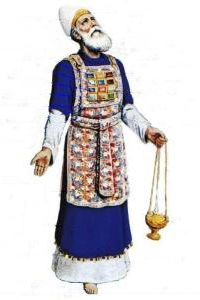
\includegraphics[width=50mm,scale=1.5]{Extras/Melchisedec.jpg}
\vspace{0.4in}  % Create a title for the document and write it in bold font
\LARGE{\textbf{\date}} % Again, do a line break
\linebreak 
% Create a subtitle \large{with Outlines, Statistics, Cross References, and Notes}
\vspace{0.5in}
\begin{flushleft}
\LARGE{Day \#45: Monday, 14 February 2022 PLAIN \\}\vspace{0.25in}
\LARGE{Numbers 13-15 Psalm 45 Proverb 14}
\end{flushleft}
\vspace{0.6in}
\bigskip

\normalsize{Xenia, Oh.\\}
\normalsize{created: \today}
\vspace{1.3in}

\end{flushright}
\end{titlepage}

\newpage 
\tableofcontents\hypertarget{TOC}{}

\hyphenation{A-bim-e-lech bre-thren E-phra-im  Gib-e-o-nites Jer-u-sa-lem through-out Phil-i-stines The-o-phil-us Am-a-le-kites ven-geance Mesh-el-e-mi-ah onan-ism Phar-a-oh thoughts grev-ous-ness Hach-a-liah adul-ter-er Shad-rach}

%%%%%%%%%%%%%%%%% EXTRA COLORS
%%%%%%%%%%%%%%%%% EXTRA COLORS
%%%%%%%%%%%%%%%%% EXTRA COLORS
\definecolor{champagne}{rgb}{0.97,0.91,0.81}
\definecolor{bone}{rgb}{0.89,0.85,0.79}

\definecolor{ForestGreen}{rgb}{0.00,0.29,0.098}
\definecolor{GIVING}{cmyk}{1,0.0,0.72,.1}

\definecolor{MLPE}{cmyk}{1,1,0,.45}
\definecolor{SOCCER}{cmyk}{.77, 0, .42, .49}
\definecolor{PAYBILL}{cmyk}{0,0.83,0.76,0.07}
\definecolor{SERMON}{cmyk}{.14,.9,0,.30} % aka seance \href{http://www.flatuicolorpicker.com/purple-cmyk-color-model/}{seance}
\definecolor{BIBLE}{cmyk}{0,.17,.74,.17}
\definecolor{WORKBLUE}{cmyk}{1, .5, 0, .6}
\definecolor{myOrange}{cmyk}{0, .4, .98, .03}
\definecolor{myTan}{cmyk}{0.0,.07,.17,.10}
\definecolor{myRed}{cmyk}{0,1,1,0}
\definecolor{myWhite}{cmyk}{0,0,0,0}
\definecolor{BLUESoD}{cmyk}{.97,.84,0,.04}
\definecolor{WHITE}{cmyk}{0,0,0,0}
\definecolor{OLDGOLD}{cmyk}{0.05,0.3,1.00,0}
\definecolor{CASTLETON}{cmyk}{1,0,0.31,0.66}
\definecolor{cadmiumgreen}{rgb}{0.0, 0.42, 0.24}
\definecolor{jungle}{rgb}{0.203,0.4882,0.1718}
\definecolor{MYGOLD}{rgb}{1,.84,0}

\definecolor{MYLIGHTGRAY}{rgb}{.85,.85,.85}

\definecolor{codegreen}{rgb}{0,0.6,0}
\definecolor{codegray}{rgb}{0.5,0.5,0.5}
\definecolor{codepurple}{rgb}{0.58,0,0.82}
\definecolor{backcolour}{rgb}{0.95,0.95,0.92}


\mdfdefinestyle{MyFrame}{%
    linecolor=blue,
    outerlinewidth=2pt,
    roundcorner=5pt,
    innertopmargin=\baselineskip,
    innerbottommargin=\baselineskip,
    innerrightmargin=10pt,
    innerleftmargin=10pt,
    backgroundcolor=gray!25!white}


\mdfdefinestyle{MyFrame2}{%
    linecolor=black,
    outerlinewidth=2pt,
    roundcorner=5pt,
    innertopmargin=\baselineskip,
    innerbottommargin=\baselineskip,
    innerrightmargin=10pt,
    innerleftmargin=10pt,
    backgroundcolor=yellow!25!white}


%%%%%
%% for PFTTIS list
%%%%%

%%% And Joseph said unto
\index[PFTTIS]{And Joseph said unto!Genesis!Gen 40:008}
\index[PFTTIS]{And Joseph said unto!Genesis!Gen 40:012}
\index[PFTTIS]{And Joseph said unto!Genesis!Gen 41:025}
\index[PFTTIS]{And Joseph said unto!Genesis!Gen 42:014}
\index[PFTTIS]{And Joseph said unto!Genesis!Gen 42:018}
\index[PFTTIS]{And Joseph said unto!Genesis!Gen 44:015}
\index[PFTTIS]{And Joseph said unto!Genesis!Gen 45:003}
\index[PFTTIS]{And Joseph said unto!Genesis!Gen 45:004}
\index[PFTTIS]{And Joseph said unto!Genesis!Gen 46:031}
\index[PFTTIS]{And Joseph said unto!Genesis!Gen 48:009}
\index[PFTTIS]{And Joseph said unto!Genesis!Gen 48:018}
\index[PFTTIS]{And Joseph said unto!Genesis!Gen 50:019}
\index[PFTTIS]{And Joseph said unto!Genesis!Gen 50:024}


%%% a shadow
\index[PFTTIS]{a shadow!1Chronicles!1Chr 029:15}
\index[PFTTIS]{a shadow!Job!Job 008:09}
\index[PFTTIS]{a shadow!Job!Job 014:02}
\index[PFTTIS]{a shadow!Job!Job 017:07}
\index[PFTTIS]{a shadow!Psalm!Psa 102:011}
\index[PFTTIS]{a shadow!Psalm!Psa 144:004}
\index[PFTTIS]{a shadow!Ecclesiastes!Eccl 006:012}
\index[PFTTIS]{a shadow!Ecclesiastes!Eccl 008:013}
\index[PFTTIS]{a shadow!Isaiah!Isa 04:006}
\index[PFTTIS]{a shadow!Isaiah!Isa 25:004}
\index[PFTTIS]{a shadow!Jonah!Jnh 04:06}
\index[PFTTIS]{a shadow!Colossians!Col 02:017}
\index[PFTTIS]{a shadow!Hebews!Heb 10:001}

%%% blessed is the man
\index[PFTTIS]{blessed is the man!Psalm!Psa 001:001}
\index[PFTTIS]{blessed is the man!Psalm!Psa 032:002}
\index[PFTTIS]{blessed is the man!Psalm!Psa 034:008}
\index[PFTTIS]{blessed is the man!Psalm!Psa 065:004}
\index[PFTTIS]{blessed is the man!Psalm!Psa 084:005}
\index[PFTTIS]{blessed is the man!Psalm!Psa 084:012}
\index[PFTTIS]{blessed is the man!Psalm!Psa 094:012}
\index[PFTTIS]{blessed is the man!Psalm!Psa 112:001}
\index[PFTTIS]{blessed is the man!Proverbs!Pro 008:034}
\index[PFTTIS]{blessed is the man!Isaiah!Isa 056:002}
\index[PFTTIS]{blessed is the man!Jeremiah!Jer 017:007}
\index[PFTTIS]{blessed is the man!Romans!Rom 004:008}
\index[PFTTIS]{blessed is the man!James!Jam 001:012}


%%% carry them
\index[PFTTIS]{carry them!Leviticus!Lev 14:045}
\index[PFTTIS]{carry them!Numbers!Num 11:012}
\index[PFTTIS]{carry them!Joshua!Jsh 04:003}
\index[PFTTIS]{carry them!1Samuel!1Sam 20:040}
\index[PFTTIS]{carry them!1Kings!1Kng 08:046}
\index[PFTTIS]{carry them!2Chronicles!2Chr 06:036}
\index[PFTTIS]{carry them!Ezra!Ezra 05:015}
\index[PFTTIS]{carry them!Isaiah!Isa 40:011}
\index[PFTTIS]{carry them!Isaiah!Isa 41:016}
\index[PFTTIS]{carry them!Isaiah!Isa 57:013}
\index[PFTTIS]{carry them!Jeremiah!Jer 20:004}
\index[PFTTIS]{carry them!Jeremiah!Jer 20:005}
\index[PFTTIS]{carry them!Jeremiah!Jer 43:012}


\index[PFTTIS]{good tidings!2Samuel!2Sam 18:027}
\index[PFTTIS]{good tidings!1Kings!1Ki 01:042}
\index[PFTTIS]{good tidings!2Kings!2Ki 07:009 (2x)}
\index[PFTTIS]{good tidings!Isaiah!Isa 40:009 (2x)}
\index[PFTTIS]{good tidings!Isaiah!Isa 41:007}
\index[PFTTIS]{good tidings!Isaiah!Isa 52:007}
\index[PFTTIS]{good tidings!Isaiah!Isa 61:001}
\index[PFTTIS]{good tidings!Nahum!Nah 01:005}
\index[PFTTIS]{good tidings!Luke!Lk 02:010}
\index[PFTTIS]{good tidings!1Thessalonians!1Thess 03:006}


%%% dead body
\index[PFTTIS]{dead body!Leviticus!Lev 21:011}
\index[PFTTIS]{dead body!Numbers!Num 06:006}
\index[PFTTIS]{dead body!Numbers!Num 09:006}
\index[PFTTIS]{dead body!Numbers!Num 09:007}
\index[PFTTIS]{dead body!Numbers!Num 09:010}
\index[PFTTIS]{dead body!Numbers!Num 09:011}
\index[PFTTIS]{dead body!Numbers!Num 09:013}
\index[PFTTIS]{dead body!Numbers!Num 09:016}
\index[PFTTIS]{dead body!2Kings!2Ki 08:005}
\index[PFTTIS]{dead body!Isaiah!Isa 26:019}
\index[PFTTIS]{dead body!Jeremiah!Jer 26:023}
\index[PFTTIS]{dead body!Jeremiah!Jer 36:030}
\index[PFTTIS]{dead body!Haggai!Hag 02:013}

%%% great sea
\index[PFTTIS]{great sea!Numbers!Num 34:006}
\index[PFTTIS]{great sea!Numbers!Num 34:007}
\index[PFTTIS]{great sea!Joshua!Jos 01:004}
\index[PFTTIS]{great sea!Joshua!Jos 09:001}
\index[PFTTIS]{great sea!Joshua!Jos 15:012}
\index[PFTTIS]{great sea!Joshua!Jos 15:047}
\index[PFTTIS]{great sea!Joshua!Jos 23:004}
\index[PFTTIS]{great sea!Ezekiel!Eze 47:010}
\index[PFTTIS]{great sea!Ezekiel!Eze 47:015}
\index[PFTTIS]{great sea!Ezekiel!Eze 47:019}
\index[PFTTIS]{great sea!Ezekiel!Eze 47:020}
\index[PFTTIS]{great sea!Ezekiel!Eze 48:028}
\index[PFTTIS]{great sea!Daniel!Dan 07:002}


%%% have forsaken me
\index[PFTTIS]{have forsaken me!Judges!Jdg 10:013}
\index[PFTTIS]{have forsaken me!1Samuel!1Sam 08:008}
\index[PFTTIS]{have forsaken me!1Kings!1Ki 11:033}
\index[PFTTIS]{have forsaken me!2Kings!2Ki 22:017}
\index[PFTTIS]{have forsaken me!2Chronicles!2Chr 12:005}
\index[PFTTIS]{have forsaken me!2Chronicles!2Chr 34:025}
\index[PFTTIS]{have forsaken me!Jeremiah!Jer 01:016}
\index[PFTTIS]{have forsaken me!Jeremiah!Jer 02:013}
\index[PFTTIS]{have forsaken me!Jeremiah!Jer 05:007}
\index[PFTTIS]{have forsaken me!Jeremiah!Jer 05:019}
\index[PFTTIS]{have forsaken me!Jeremiah!Jer 16:011 (2x)}
\index[PFTTIS]{have forsaken me!Jeremiah!Jer 19:004}

%%% no king
\index[PFTTIS]{no king!Judges!Jdg 17:06}
\index[PFTTIS]{no king!Judges!Jdg 18:01}
\index[PFTTIS]{no king!Judges!Jdg 19:01}
\index[PFTTIS]{no king!Judges!Jdg 21:25}
\index[PFTTIS]{no king!1Kings!1Ki 22:47}
\index[PFTTIS]{no king!2Kings!2Ki 23:25}
\index[PFTTIS]{no king!Nehemiah!Neh 13:26}
\index[PFTTIS]{no king!Psalms!Psa 033:016}
\index[PFTTIS]{no king!Proverbs!Pro 30:27}
\index[PFTTIS]{no king!Daniel!Dan 02:10}
\index[PFTTIS]{no king!Hosea!Hos 10:03}
\index[PFTTIS]{no king!Micah!Mic 04:09}
\index[PFTTIS]{no king!John!Jhn 19:15}


%%% rebellious house
\index[PFTTIS]{rebellious house!Exodus!Exo 02:005}
\index[PFTTIS]{rebellious house!Exodus!Exo 02:006}
\index[PFTTIS]{rebellious house!Exodus!Exo 02:008}
\index[PFTTIS]{rebellious house!Exodus!Exo 03:009}
\index[PFTTIS]{rebellious house!Exodus!Exo 03:026}
\index[PFTTIS]{rebellious house!Exodus!Exo 03:027}
\index[PFTTIS]{rebellious house!Exodus!Exo 12:002 (2x)}
\index[PFTTIS]{rebellious house!Exodus!Exo 12:003}
\index[PFTTIS]{rebellious house!Exodus!Exo 12:009}
\index[PFTTIS]{rebellious house!Exodus!Exo 12:025}
\index[PFTTIS]{rebellious house!Exodus!Exo 17:012}
\index[PFTTIS]{rebellious house!Exodus!Exo 24:003}

%%% seek him
\index[PFTTIS]{seek him!Deuteronomy!Deu 04:029}\index[PFTTIS]{seek him!1Samuel!1Sam 23:025}
\index[PFTTIS]{seek him!1Chronicles!1Chr 28:009}
\index[PFTTIS]{seek him!2Chronicles!1Chr 15:002}
\index[PFTTIS]{seek him!Ezra!Ezr 08:022}
\index[PFTTIS]{seek him!Psalms!Psa 022:026}
\index[PFTTIS]{seek him!Psalms!Psa 024:006}
\index[PFTTIS]{seek him!Psalms!Psa 119:002}
\index[PFTTIS]{seek him!SoS!SoS 03:002}
\index[PFTTIS]{seek him!SoS!SoS 06:001}
\index[PFTTIS]{seek him!Hosea!Hos 07:010}
\index[PFTTIS]{seek him!Amos!Amo 05:008}
\index[PFTTIS]{seek him!Hebrews!Heb 11:0063}


%%% seek ye
\index[PFTTIS]{seek ye!Isaiah!Isa 34:016}
\index[PFTTIS]{seek ye!Isaiah!Isa 45:019}
\index[PFTTIS]{seek ye!Isaiah!Isa 55:006}
\index[PFTTIS]{seek ye!Amos!Amos 5:004}
\index[PFTTIS]{seek ye!John!John 1:38}
\index[PFTTIS]{seek ye!John!John 18:4}
\index[PFTTIS]{seek ye!John!John 18:7}
\index[PFTTIS]{seek ye!Matthew!Matt 6:33}
\index[PFTTIS]{seek ye!Numbers!Num 16:10}
\index[PFTTIS]{seek ye!Luke!Luke 12:31}
\index[PFTTIS]{seek ye!Luke!Luke 24:5}
\index[PFTTIS]{seek ye!Psalm!Psa 27:8}
\index[PFTTIS]{seek ye!Zephaniah!Zeph 2:3}

%%% the uncircumcised
\index[PFTTIS]{the uncircumcised!Genesis!Gen 17:014}
\index[PFTTIS]{the uncircumcised!Judges!Jdg 14:003}
\index[PFTTIS]{the uncircumcised!Judges!Jdg 15:018}
\index[PFTTIS]{the uncircumcised!2Samuel!2Sam 01:020}
\index[PFTTIS]{the uncircumcised!Isaiah!Isa 02:001}
\index[PFTTIS]{the uncircumcised!Jeremiah!Jer 09:025}
\index[PFTTIS]{the uncircumcised!Ezekiel!Eze 28:010}
\index[PFTTIS]{the uncircumcised!Ezekiel!Eze 31:018}
\index[PFTTIS]{the uncircumcised!Ezekiel!Eze 32:019}
\index[PFTTIS]{the uncircumcised!Ezekiel!Eze 32:027}
\index[PFTTIS]{the uncircumcised!Ezekiel!Eze 32:028}
\index[PFTTIS]{the uncircumcised!Ezekiel!Eze 32:029}
\index[PFTTIS]{the uncircumcised!Ezekiel!Eze 32:032}

%%% worship him
\index[PFTTIS]{worship him!Psalms!Psa 97:007}
\index[PFTTIS]{worship him!Zephaniah!Zeph 02:011}
\index[PFTTIS]{worship him!Matthew!Matt 02:002}
\index[PFTTIS]{worship him!Matthew!Matt 02:008}
\index[PFTTIS]{worship him!John!John 04:023}
\index[PFTTIS]{worship him!John!John 04:024 (2x)} 
\index[PFTTIS]{worship him!Acts!Acts 17:023}
\index[PFTTIS]{worship him!Hebrews!Heb 01:006}
\index[PFTTIS]{worship him!Revelation!Rev 04:010}
\index[PFTTIS]{worship him!Revelation!Rev 13:008}
\index[PFTTIS]{worship him!Revelation!Rev 14:007}
\index[PFTTIS]{worship him!Revelation!Rev 19:010}


%%%%%
%% for PFTTIS list
%%%%%

%%% afflictions
\index[WFTTIS]{afflictions!Psalms!Psa 34:019}
\index[WFTTIS]{afflictions!Psalms!Psa 132:001}
\index[WFTTIS]{afflictions!Acts!Acts 07:010}
\index[WFTTIS]{afflictions!Acts!Acts 20:023}
\index[WFTTIS]{afflictions!2Corinthians!2Cor 06:004}
\index[WFTTIS]{afflictions!Colossians!Col 01:024}
\index[WFTTIS]{afflictions!1Thessalonians!1Thess 03:003}
\index[WFTTIS]{afflictions!2Timothy!2Tim 01:008}
\index[WFTTIS]{afflictions!2Timothy!2Tim 03:011}
\index[WFTTIS]{afflictions!2Timothy!2Tim 04:005}
\index[WFTTIS]{afflictions!Hebrews!Heb 10:032}
\index[WFTTIS]{afflictions!Hebrews!Heb 10:033}
\index[WFTTIS]{afflictions!1Peter!1Pet 05:009}

%%% acsend
\index[WFTTIS]{acsend!Joshua!Jos 06:05}
\index[WFTTIS]{acsend!Psalm!Psa 024:003}
\index[WFTTIS]{acsend!Psalm!Psa 135:007}
\index[WFTTIS]{acsend!Psalm!Psa 139:008}
\index[WFTTIS]{acsend!Isaiah!Isa 14:013}
\index[WFTTIS]{acsend!Isaiah!Isa 14:014}
\index[WFTTIS]{acsend!Jeremiah!Jer 10:013}
\index[WFTTIS]{acsend!Jeremiah!Jer 51:016}
\index[WFTTIS]{acsend!Ezekiel!Eze 38:009}
\index[WFTTIS]{acsend!John!John 06:062}
\index[WFTTIS]{acsend!John!John 20:017}
\index[WFTTIS]{acsend!Romans!Rom 10:006}
\index[WFTTIS]{acsend!Revelation!Rev 17:008}

%%% Assyrian
\index[WFTTIS]{Assyrian!Isaiah!Isa 10:005}
\index[WFTTIS]{Assyrian!Isaiah!Isa 10:024}
\index[WFTTIS]{Assyrian!Isaiah!Isa 14:025}
\index[WFTTIS]{Assyrian!Isaiah!Isa 19:023}
\index[WFTTIS]{Assyrian!Isaiah!Isa 23:013}
\index[WFTTIS]{Assyrian!Isaiah!Isa 30:031}
\index[WFTTIS]{Assyrian!Isaiah!Isa 31:008}
\index[WFTTIS]{Assyrian!Isaiah!Isa 52:004}
\index[WFTTIS]{Assyrian!Ezekiel!Eze 31:003}
\index[WFTTIS]{Assyrian!Hosea!Hos 05:013}
\index[WFTTIS]{Assyrian!Hosea!Hos 11:005}
\index[WFTTIS]{Assyrian!Micah!Hos 05:005}
\index[WFTTIS]{Assyrian!Micah!Hos 05:006}

%%% blot
\index[WFTTIS]{blot!Exodus!Exo 32:032}
\index[WFTTIS]{blot!Exodus!Exo 32:033}
\index[WFTTIS]{blot!Numbers!Num 05:026}
\index[WFTTIS]{blot!Deuteronomy!Deut 09:014}
\index[WFTTIS]{blot!Deuteronomy!Deut 25:019}
\index[WFTTIS]{blot!Deuteronomy!Deut 29:020}
\index[WFTTIS]{blot!2Kings!2Ki 14:027}
\index[WFTTIS]{blot!Job!Job 31:007}
\index[WFTTIS]{blot!Psalms!Psa 51:001}
\index[WFTTIS]{blot!Psalms!Psa 51:009}
\index[WFTTIS]{blot!Proverbs!Pro 09:007}
\index[WFTTIS]{blot!Jeremiah!Jer 18:023}
\index[WFTTIS]{blot!Revelation!Rev 03:005}


%%% chain
\index[WFTTIS]{chain!Genesis!Gen 41:042}
\index[WFTTIS]{chain!1Kings!1Ki 07:017}
\index[WFTTIS]{chain!Psalms!Psa 73:006}
\index[WFTTIS]{chain!SoS!Sos 04:009}
\index[WFTTIS]{chain!Lamentations!Lam 03:007}
\index[WFTTIS]{chain!Ezekiel!Eze 07:023}
\index[WFTTIS]{chain!Ezekiel!Eze 16:011}
\index[WFTTIS]{chain!Daniel!Dan 05:007}
\index[WFTTIS]{chain!Daniel!Dan 05:016}
\index[WFTTIS]{chain!Daniel!Dan 05:029}
\index[WFTTIS]{chain!Acts!Acts 28:020}
\index[WFTTIS]{chain!2Timothy!2Tim 01:016}
\index[WFTTIS]{chain!Revelation!Rev 20:001}


%%% controversy
\index[WFTTIS]{controversy!Deuteronomy!Deu 17:008}
\index[WFTTIS]{controversy!Deuteronomy!Deu 19:017}
\index[WFTTIS]{controversy!Deuteronomy!Deu 21:005}
\index[WFTTIS]{controversy!Deuteronomy!Deu 25:001}
\index[WFTTIS]{controversy!2Samuel!2Sam 15:002}
\index[WFTTIS]{controversy!Isaiah!Isa 34:008}
\index[WFTTIS]{controversy!Jeremiah!Jer 25:031}
\index[WFTTIS]{controversy!Ezekiel!Eze 44:024}
\index[WFTTIS]{controversy!Hosea!Hos 04:001}
\index[WFTTIS]{controversy!Hosea!Hos 12:002}
\index[WFTTIS]{controversy!Micah!Mic 06:002 (2x)}
\index[WFTTIS]{controversy!1Timothy!1Tim 03:016}


%%% Dagon/Dagon's
\index[WFTTIS]{Dagon!Judges!Jdg 16:023}
\index[WFTTIS]{Dagon!1Samuel!1Sam 05:002 (2x)}
\index[WFTTIS]{Dagon!1Samuel!1Sam 05:003 (2x)}
\index[WFTTIS]{Dagon!1Samuel!1Sam 05:004 (3x)}
\index[WFTTIS]{Dagon!1Samuel!1Sam 05:005 (3x)}
\index[WFTTIS]{Dagon!1Samuel!1Sam 05:007}
\index[WFTTIS]{Dagon!1Chronicles!1Chr 10:010}

%%% disobedient
\index[WFTTIS]{disobedient!1Kings!1Ki 13:026}
\index[WFTTIS]{disobedient!Nehemiah!Neh 09:026}
\index[WFTTIS]{disobedient!Luke!Luke 01:017}
\index[WFTTIS]{disobedient!Acts!Acts 26:019}
\index[WFTTIS]{disobedient!Romans!Rom 01:030}
\index[WFTTIS]{disobedient!Romans!Rom 10:021}
\index[WFTTIS]{disobedient!1Timothy!1Tim 01:009}
\index[WFTTIS]{disobedient!2Timothy!2Tim 03:002}
\index[WFTTIS]{disobedient!Titus!Titus 01:016}
\index[WFTTIS]{disobedient!Titus!Titus 03:003}
\index[WFTTIS]{disobedient!1Peter!1Pet 02:007}
\index[WFTTIS]{disobedient!1Peter!1Pet 02:008}
\index[WFTTIS]{disobedient!1Peter!1Pet 03:020}


%%% doubt
\index[WFTTIS]{doubt!Genesis!Gen 37:033}
\index[WFTTIS]{doubt!Deuteronomy!Deu 28:066}
\index[WFTTIS]{doubt!Job!Job 12:002}
\index[WFTTIS]{doubt!Matthew!Matt 14:031}
\index[WFTTIS]{doubt!Matthew!Matt 21:021}
\index[WFTTIS]{doubt!Mark!Mk 11:023}
\index[WFTTIS]{doubt!Luke!Lk 11:020}
\index[WFTTIS]{doubt!John!Jhn 10:024}
\index[WFTTIS]{doubt!Acts!Acts 02:012}
\index[WFTTIS]{doubt!Acts!Acts 28:004}
\index[WFTTIS]{doubt!1Corinthians!1Cor 09:010}
\index[WFTTIS]{doubt!Galatians!Gal 04:020}
\index[WFTTIS]{doubt!1John!1Jhn 02:019}


%%% dungeon
\index[WFTTIS]{dungeon!Genesis!Gen 40:015}
\index[WFTTIS]{dungeon!Genesis!Gen 41:014}
\index[WFTTIS]{dungeon!Exodus!Exo 12:029}
\index[WFTTIS]{dungeon!Jeremiah!Jer 37:016}
\index[WFTTIS]{dungeon!Jeremiah!Jer 38:006 (2x)}
\index[WFTTIS]{dungeon!Jeremiah!Jer 38:007}
\index[WFTTIS]{dungeon!Jeremiah!Jer 38:009}
\index[WFTTIS]{dungeon!Jeremiah!Jer 38:010}
\index[WFTTIS]{dungeon!Jeremiah!Jer 38:011}
\index[WFTTIS]{dungeon!Jeremiah!Jer 38:013}
\index[WFTTIS]{dungeon!Lamentations!Lam 03:053}
\index[WFTTIS]{dungeon!Lamentations!Lam 03:055}


%%% error
\index[WFTTIS]{error!2Samuel!2Sam 06:007}
\index[WFTTIS]{error!Job!Job 19:004}
\index[WFTTIS]{error!Ecclesiastes!Ecc 05:006}
\index[WFTTIS]{error!Ecclesiastes!Ecc 10:005}
\index[WFTTIS]{error!Isaiah!Isa 32:006}
\index[WFTTIS]{error!Daniel!Dan 06:004}
\index[WFTTIS]{error!Matthew!Matt 27:064}
\index[WFTTIS]{error!Romans!Rom 01:027}
\index[WFTTIS]{error!James!Jam 05:020}
\index[WFTTIS]{error!2Peter!2Pet 02:018}
\index[WFTTIS]{error!2Peter!2Pet 03:017}
\index[WFTTIS]{error!1John!1Jn 04:006}
\index[WFTTIS]{error!Jude!Jude 01:011}

%%% fourish
\index[WFTTIS]{fourish!Psalms!Psa 072:007}
\index[WFTTIS]{fourish!Psalms!Psa 072:016}
\index[WFTTIS]{fourish!Psalms!Psa 092:007}
\index[WFTTIS]{fourish!Psalms!Psa 092:012}
\index[WFTTIS]{fourish!Psalms!Psa 092:013}
\index[WFTTIS]{fourish!Psalms!Psa 132:018}
\index[WFTTIS]{fourish!Proverbs!Pro 11:28}
\index[WFTTIS]{fourish!Proverbs!Pro 14:11}
\index[WFTTIS]{fourish!Ecclesiastes!Ecc 12:05}
\index[WFTTIS]{fourish!SongOfSolomon!SOS 07:12}
\index[WFTTIS]{fourish!Isaiah!Isa 17:11}
\index[WFTTIS]{fourish!Isaiah!Isa 66:14}
\index[WFTTIS]{fourish!Ezekiel!Eze 17:24}




%%% giants
\index[WFTTIS]{giants!Genesis!Gen 06:004}
\index[WFTTIS]{giants!Numbers!Num 13:033}
\index[WFTTIS]{giants!Deuteronomy!Deut 02:011}
\index[WFTTIS]{giants!Deuteronomy!Deut 02:021}
\index[WFTTIS]{giants!Deuteronomy!Deut 03:011}
\index[WFTTIS]{giants!Deuteronomy!Deut 03:013}
\index[WFTTIS]{giants!Joshua!Josh 12:004}
\index[WFTTIS]{giants!Joshua!Josh 13:012}
\index[WFTTIS]{giants!Joshua!Josh 15:008}
\index[WFTTIS]{giants!Joshua!Josh 17:015}
\index[WFTTIS]{giants!Joshua!Josh 16:016}

%%% good man
\index[WFTTIS]{good man!2 Samuel!2Sa 18:27}
%(1) Psalms 37:23 [5]
%(1) Psalms 112:5 [2]
%(1) Proverbs 12:2 [2]
%(1) Proverbs 13:22 [2]
%(1) Proverbs 14:14 [14]
%(1) Micah 7:2 [2]
%(1) Matthew 12:35 [2]
%(1) Luke 6:45 [2]
%(1) Luke 23:50 [15]
%(1) John 7:12 [17]
%(1) Acts 11:24 [5]
%(1) Romans 5:7 [14]

%%% Hinnom
\index[WFTTIS]{Hinnom!Joshua!Jsh 15:008}
\index[WFTTIS]{Hinnom!Joshua!Jsh 18:016}
\index[WFTTIS]{Hinnom!2Kings!2Ki 23:010}
\index[WFTTIS]{Hinnom!2Chronicles!2Chr 28:003}
\index[WFTTIS]{Hinnom!2Chronicles!2Chr 33:006}
\index[WFTTIS]{Hinnom!Nehemiah!Neh 11:030}
\index[WFTTIS]{Hinnom!Jeremiah!Jer 07:031}
\index[WFTTIS]{Hinnom!Jeremiah!Jer 07:032}
\index[WFTTIS]{Hinnom!Jeremiah!Jer 19:002}
\index[WFTTIS]{Hinnom!Jeremiah!Jer 19:006}
\index[WFTTIS]{Hinnom!Jeremiah!Jer 32:035}

%%% inclined
\index[WFTTIS]{inclined!Judges!Jdg 09:003}
\index[WFTTIS]{inclined!Psalms!Psa 040:001}
\index[WFTTIS]{inclined!Psalms!Psa 116:002}
\index[WFTTIS]{inclined!Psalms!Psa 119:112}
\index[WFTTIS]{inclined!Proverbs!Pro 05:13}
\index[WFTTIS]{inclined!Jeremiah!Jer 07:24}
\index[WFTTIS]{inclined!Jeremiah!Jer 07:26}
\index[WFTTIS]{inclined!Jeremiah!Jer 11:08}
\index[WFTTIS]{inclined!Jeremiah!Jer 17:23}
\index[WFTTIS]{inclined!Jeremiah!Jer 25:04}
\index[WFTTIS]{inclined!Jeremiah!Jer 34:14}
\index[WFTTIS]{inclined!Jeremiah!Jer 35:15}
\index[WFTTIS]{inclined!Jeremiah!Jer 44:05}


%%% laughed
\index[WFTTIS]{laughed!Genesis!Gen 17:017}
\index[WFTTIS]{laughed!Genesis!Gen 18:012}
\index[WFTTIS]{laughed!Genesis!Gen 18:015}
\index[WFTTIS]{laughed!2Kings!2Ki 19:021}
\index[WFTTIS]{laughed!2Chronicles!2Chr 30:010}
\index[WFTTIS]{laughed!Nehemiah!Neh 02:019}
\index[WFTTIS]{laughed!Job!Job 12:004}
\index[WFTTIS]{laughed!Job!Job 29:024}
\index[WFTTIS]{laughed!Isaiah!Isa 37:022}
\index[WFTTIS]{laughed!Ezekiel!Ezek 23:032}
\index[WFTTIS]{laughed!Matthew!Matt 09:024}
\index[WFTTIS]{laughed!Mark!Mk 05:040}
\index[WFTTIS]{laughed!Luke!Lk 08:053}

%%% liar
\index[WFTTIS]{liar!Job!Job 24:025}
\index[WFTTIS]{liar!Proverbs!Pro 17:004}
\index[WFTTIS]{liar!Proverbs!Pro 19:022}
\index[WFTTIS]{liar!Proverbs!Pro 30:006}
\index[WFTTIS]{liar!Jeremiah!Jer 15:018}
\index[WFTTIS]{liar!John!Jhn 08:044}
\index[WFTTIS]{liar!John!Jhn 08:055}
\index[WFTTIS]{liar!Romans!Rom 03:004}
\index[WFTTIS]{liar!1John!1Jhn 01:010}
\index[WFTTIS]{liar!1John!1Jhn 02:004}
\index[WFTTIS]{liar!1John!1Jhn 02:022}
\index[WFTTIS]{liar!1John!1Jhn 04:020}
\index[WFTTIS]{liar!1John!1Jhn 05:010}

%%% palsy
\index[WFTTIS]{palsy!Matthew!Matt 04:024}
\index[WFTTIS]{palsy!Matthew!Matt 08:006}
\index[WFTTIS]{palsy!Matthew!Matt 09:002}
\index[WFTTIS]{palsy!Matthew!Matt 09:006}
\index[WFTTIS]{palsy!Mark!Mk 02:003}
\index[WFTTIS]{palsy!Mark!Mk 02:004}
\index[WFTTIS]{palsy!Mark!Mk 02:005}
\index[WFTTIS]{palsy!Mark!Mk 02:009}
\index[WFTTIS]{palsy!Mark!Mk 02:010}
\index[WFTTIS]{palsy!Luke!Lk 05:018}
\index[WFTTIS]{palsy!Luke!Lk 05:024}
\index[WFTTIS]{palsy!Acts!Acts 09:033}

%%% Profitable
\index[WFTTIS]{profitable!Job!Job 22:002 (2x)}
\index[WFTTIS]{profitable!Ecclesiastes!Ecc 10:010}
\index[WFTTIS]{profitable!Isaiah!Isa 44:010}
\index[WFTTIS]{profitable!Jeremiah!Jer 13:007}
\index[WFTTIS]{profitable!Matthew!Matt 05:029}
\index[WFTTIS]{profitable!Matthew!Matt 05:030}
\index[WFTTIS]{profitable!Acts!Acts 20:020}
\index[WFTTIS]{profitable!1Timothy!1Tim 04:008}
\index[WFTTIS]{profitable!2Timothy!2Tim 03:016}
\index[WFTTIS]{profitable!2Timothy!2Tim 04:011}
\index[WFTTIS]{profitable!Titus!Titus 03:008}
\index[WFTTIS]{profitable!Philemon!Phlm 01:011}

%%% Rechab
\index[WFTTIS]{Rechab!2Samuel!2Sam 04:002}
\index[WFTTIS]{Rechab!2Samuel!2Sam 04:005}
\index[WFTTIS]{Rechab!2Samuel!2Sam 04:006}
\index[WFTTIS]{Rechab!2Samuel!2Sam 04:009}
\index[WFTTIS]{Rechab!2KIngs!2Ki 10:015}
\index[WFTTIS]{Rechab!2KIngs!2Ki 10:023}
\index[WFTTIS]{Rechab!1Chronicles!1Chr 02:055}
\index[WFTTIS]{Rechab!Nehemiah!Neh 03:014}
\index[WFTTIS]{Rechab!Jeremiah!Jer 35:006}
\index[WFTTIS]{Rechab!Jeremiah!Jer 35:008}
\index[WFTTIS]{Rechab!Jeremiah!Jer 35:014}
\index[WFTTIS]{Rechab!Jeremiah!Jer 35:016}
\index[WFTTIS]{Rechab!Jeremiah!Jer 35:019}

%%% serpents
\index[WFTTIS]{serpents!Exodus!Exo 07:012}
\index[WFTTIS]{serpents!Numbers!Num 21:006}
\index[WFTTIS]{serpents!Numbers!Num 21:007}
\index[WFTTIS]{serpents!Deuteronomy!Deu 08:015}
\index[WFTTIS]{serpents!Deuteronomy!Deu 32:024}
\index[WFTTIS]{serpents!Jeremiah!Jer 08:017}
\index[WFTTIS]{serpents!Matthew!Matt 10:016}
\index[WFTTIS]{serpents!Matthew!Matt 23:033}
\index[WFTTIS]{serpents!Mark!Mk 16:018}
\index[WFTTIS]{serpents!Luke!Lk 10:019}
\index[WFTTIS]{serpents!1Corinthians!1Cor 10:009}
\index[WFTTIS]{serpents!James!Jas 03:007}
\index[WFTTIS]{serpents!Revelation!Rev 09:019}

%%% short
\index[WFTTIS]{short!Numbers!Num 11:023}
\index[WFTTIS]{short!2Kings!2Ki 10:032}
\index[WFTTIS]{short!Job!Job 17:012}
\index[WFTTIS]{short!Job!Job 20:005}
\index[WFTTIS]{short!Psalms!Psa 89:047}
\index[WFTTIS]{short!Romans!Rom 03:023}
\index[WFTTIS]{short!Romans!Rom 09:028  (2x)}
\index[WFTTIS]{short!1Corinthians!1Cor 07:029}
\index[WFTTIS]{short!1Thessalonians!1Thess 02:017}
\index[WFTTIS]{short!Hebrews!Heb 04:001}
\index[WFTTIS]{short!Revelation!Rev 12:012}
\index[WFTTIS]{short!Revelation!Rev 17:010}

%%% smiteth
\index[WFTTIS]{smiteth!Exodus!Exo 21:012}
\index[WFTTIS]{smiteth!Exodus!Exo 21:15}
\index[WFTTIS]{smiteth!Deuteronomy!Dt 25:11}
\index[WFTTIS]{smiteth!Deuteronomy!Dt 27:24}
\index[WFTTIS]{smiteth!Joshua!Jsh 15:16}
\index[WFTTIS]{smiteth!Judges!Jdg 15:16}
\index[WFTTIS]{smiteth!2 Samuel!2Sa 05:08}
\index[WFTTIS]{smiteth!1Chronicles!1Chr 11:06}
\index[WFTTIS]{smiteth!Job!1Chr 26:12}
\index[WFTTIS]{smiteth!Isaiah!Isa 09:13}
\index[WFTTIS]{smiteth!Lamentations!Lam 03:30}
\index[WFTTIS]{smiteth!Ezekiel!Eze 07:09}
\index[WFTTIS]{smiteth!Luke!Lk 06:29}



%%% vanities
\index[WFTTIS]{vanities!Deuteronomy!Deut 21:021}
\index[WFTTIS]{vanities!1Kings!1Ki 16:013}
\index[WFTTIS]{vanities!1Kings!1Ki 16:026}
\index[WFTTIS]{vanities!Psalms!Psa 031:006}
\index[WFTTIS]{vanities!Ecclesiastes!Ecc 01:002 (2x)}
\index[WFTTIS]{vanities!Ecclesiastes!Ecc 05:007}
\index[WFTTIS]{vanities!Ecclesiastes!Ecc 12:008}
\index[WFTTIS]{vanities!Jeremiah!Jer 08:019}
\index[WFTTIS]{vanities!Jeremiah!Jer 10:008}
\index[WFTTIS]{vanities!Jeremiah!Jer 14:022}
\index[WFTTIS]{vanities!Jonah!Jnh 02:008}
\index[WFTTIS]{vanities!Acts!Acts 14:015}



%%%%%
%% for PFTTIS list
%%%%%

%%% worm
\index[WFITV]{worm!Exodus!Exo 16:024}
\index[WFITV]{worm!Job!Job 17:014}
\index[WFITV]{worm!Job!Job 24:029}
\index[WFITV]{worm!Job!Job 25:005 (2x)}
\index[WFITV]{worm!Psalms!Psa 022:006}
\index[WFITV]{worm!Isaiah!Isa 14:011}
\index[WFITV]{worm!Isaiah!Isa 41:014}
\index[WFITV]{worm!Isaiah!Isa 51:008}
\index[WFITV]{worm!Isaiah!Isa 66:024}
\index[WFITV]{worm!Jonah!Jnh 04:007}
\index[WFITV]{worm!Mark!Mk 09:044}
\index[WFITV]{worm!Mark!Mk 09:046}
\index[WFITV]{worm!Mark!Mk 09:048}


%\subsubsection{Title}
%\textbf{Introduction:} Isaiah 46 
%\index[speaker]{Speaker!Isaiah 49 (Title}
%\index[series]{Book (Speaker)!IPassage (Title)}
%\index[date]{2017/07/09!Isaiah 49 (Title)}
%\begin{compactenum}[I.]
%    \item  \textbf{Point} \index[scripture]{Isaiah!IPassage} (IPassage)
%\end{compactenum}




  



\chapter{Numbers 13}

\begin{figure}
  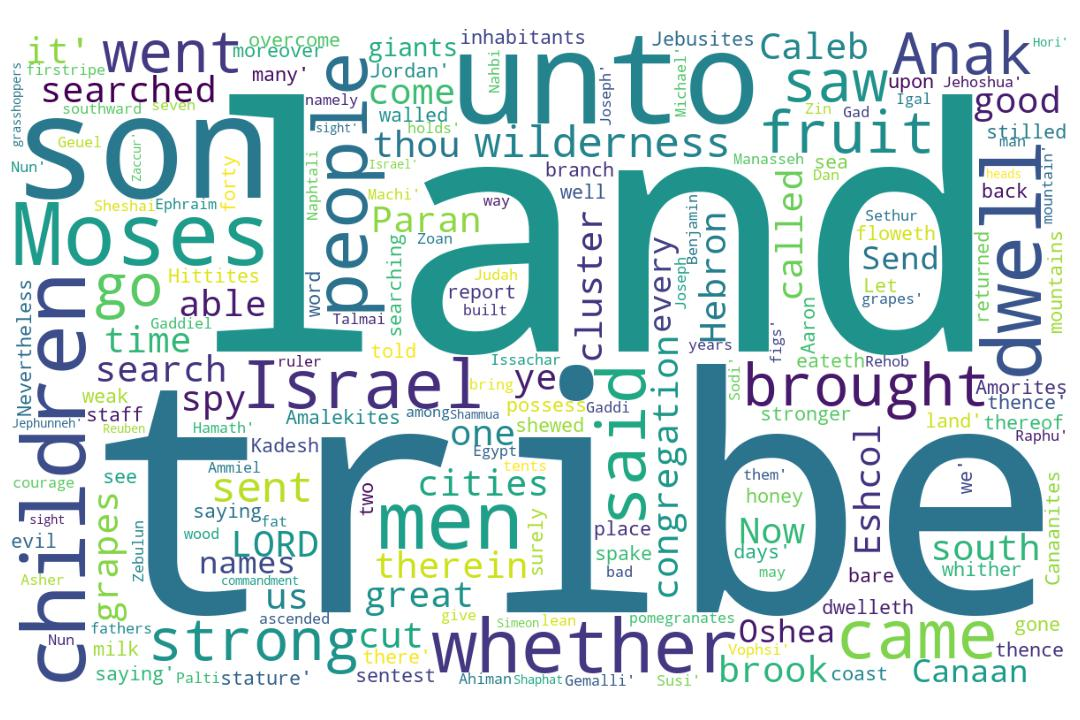
\includegraphics[width=\linewidth]{04OT-Numbers/Numbers13-WordCloud.jpg}
  \caption{Numbers 13 Word Cloud}
  \label{fig:Numbers 13 word Cloud}
\end{figure}



\marginpar{\scriptsize \centering \fcolorbox{bone}{lime}{\textbf{A 40-YEAR MISTAKE}}\\ (Numbers 13:1-33) \begin{compactenum}[I.][8]
    \item An \textbf{Inspection Tour} \index[scripture]{Numbers!Num 13:17}(Num 13:17) 
    \item An \textbf{Important Test} \index[scripture]{Numbers!Num 13:25}(Num 13:25) 
    \item \textbf{Impenetrable Towns} \index[scripture]{Numbers!Num 13:28}(Num 13:28) 
    \item \textbf{Insolent Transgressors} \index[scripture]{Numbers!Num 13:31}(Num 13:31) 
    \item People \textbf{Impressive \& Tall} \index[scripture]{Numbers!Num 13:32, 33}(Num 13:32, 33) 
    \item As \textbf{Insignificant Tourists} \index[scripture]{Numbers!Num 13:33}(Num 13:33) 
    \item An \textbf{Instructive Time} %\index[scripture]{Numbers!Numbers 13:17}(Numbers 13:17) 
\end{compactenum}}


\marginpar{\scriptsize \centering \fcolorbox{bone}{yellow}{\textbf{REBELLION AT KADESH}}\\ (Numbers 13:1-33) \begin{compactenum}[I.][8]
   \item The \textbf{Sending}  \index[scripture]{Numbers!Num 13:01}    (Num 13:1) 
   \item The \textbf{Search} \index[scripture]{Numbers!Num 13:01}  \index[scripture]{Numbers!Num 13:21}  \index[scripture]{Numbers!Num 13:25}\index[scripture]{Numbers!Num 13:32}  (Num 13:1, 21, 25, 32) 
   \item The \textbf{Sons}  \index[scripture]{Numbers!Num 13:04--15}    (Num 13:4--15) 
    \item The \textbf{Strength} of the Enemy \index[scripture]{Numbers!Num 13:18}\index[scripture]{Numbers!Num 13:28} \index[scripture]{Numbers!Num 13:31}  (Num 13:18, 28, 31) 
   \item The \textbf{Stature}  \index[scripture]{Numbers!Num 13:32}    (Num 13:32) 
   \item The \textbf{Sight}  of the Spies \index[scripture]{Numbers!Num 13:33}    (Num 13:33) 
  \item The \textbf{Significance} of Unbelief %\index[scripture]{Numbers!Num 13:01}    (Numbers 13:1) 
\end{compactenum}}

\marginpar{\scriptsize \centering \fcolorbox{bone}{black}{\textbf{\textcolor[cmyk]{0,0,0,0}{THE SPIES}}}\\ (Numbers 13:1-33) 
 \begin{compactenum}[I.][8]
   \item \textbf{Required} for the Mission \index[scripture]{Numbers!Num 13:02}    (Num 13:2) 
   \item \textbf{Represented} the Tribes \index[scripture]{Numbers!Num 13:02}    (Num 13:2) 
   \item \textbf{Recounted} the Enemies\index[scripture]{Numbers!Num 13:27--28}    (Num 13:27--28)
   \item \textbf{Rebelled}  \index[scripture]{Numbers!Num 13:31}    (Num 13:31)
   \item \textbf{Disregarded} the LORD \index[scripture]{Numbers!Num 13:31}    (Num 13:31)
   \item \textbf{Ruined} the chances to Enter the Land  ... for 40 years, and the death of over 600,000 men plus women and children and the strangers who were with them
   \item Didn't \textbf{Recognize} what they had with them
\end{compactenum}}

\marginpar{\scriptsize \centering \fcolorbox{bone}{blue}{\textcolor{white}{\textbf{THE SPIES DID NOT SEE}}}\\ (Numbers 13:1-33) 
 \begin{compactenum}[I.][8]
   \item The \textbf{Goodness} that Awaited \index[scripture]{Numbers!Num 13:32}    (Numbers 13:32) 
   \item The \textbf{Giants} Annihilated
   \item A \textbf{God} who is Awesome -- Bigger than the Giants 
   \item The \textbf{Grief} After their rebellion -- a defeat in the next chapter, a 40-year wait
   \item The \textbf{Guidance} that was Available
   \item  \textbf{Great} Victories Ahead
   \item The \textbf{Glory} of God Above all Else
\end{compactenum}}


\footnote{\textcolor[cmyk]{0.99998,1,0,0}{\hyperlink{TOC}{Return to end of Table of Contents.}}}\footnote{\href{https://audiobible.com/bible/numbers_13.html}{\textcolor[cmyk]{0.99998,1,0,0}{Numbers 13 Audio}}}\textcolor[cmyk]{0.99998,1,0,0}{And the LORD spake unto Moses, saying,}
[2] \textcolor[cmyk]{0.99998,1,0,0}{Send thou men, that they may search the land of Canaan, which I give unto the children of Israel: of every tribe of their fathers shall ye send a man, every one a ruler among them.}
[3] \textcolor[cmyk]{0.99998,1,0,0}{And Moses by the commandment of the LORD sent them from the wilderness of Paran: all those men \emph{were} heads of the children of Israel.}
[4] \textcolor[cmyk]{0.99998,1,0,0}{And these \emph{were} their names: of the tribe of Reuben, Shammua the \fcolorbox{bone}{bone}{son} of Zaccur.}
[5] \textcolor[cmyk]{0.99998,1,0,0}{Of the tribe of Simeon, Shaphat the \fcolorbox{bone}{bone}{son} of Hori.}
[6] \textcolor[cmyk]{0.99998,1,0,0}{Of the tribe of Judah, Caleb the \fcolorbox{bone}{bone}{son} of Jephunneh.}
[7] \textcolor[cmyk]{0.99998,1,0,0}{Of the tribe of Issachar, Igal the \fcolorbox{bone}{bone}{son} of Joseph.}
[8] \textcolor[cmyk]{0.99998,1,0,0}{Of the tribe of Ephraim, Oshea the \fcolorbox{bone}{bone}{son} of Nun.}
[9] \textcolor[cmyk]{0.99998,1,0,0}{Of the tribe of Benjamin, Palti the \fcolorbox{bone}{bone}{son} of Raphu.}
[10] \textcolor[cmyk]{0.99998,1,0,0}{Of the tribe of Zebulun, Gaddiel the \fcolorbox{bone}{bone}{son} of Sodi.}
[11] \textcolor[cmyk]{0.99998,1,0,0}{Of the tribe of Joseph, \emph{namely}, of the tribe of Manasseh, Gaddi the \fcolorbox{bone}{bone}{son} of Susi.}
[12] \textcolor[cmyk]{0.99998,1,0,0}{Of the tribe of Dan, Ammiel the \fcolorbox{bone}{bone}{son} of Gemalli.}
[13] \textcolor[cmyk]{0.99998,1,0,0}{Of the tribe of Asher, Sethur the \fcolorbox{bone}{bone}{son} of Michael.}
[14] \textcolor[cmyk]{0.99998,1,0,0}{Of the tribe of Naphtali, Nahbi the \fcolorbox{bone}{bone}{son} of Vophsi.}
[15] \textcolor[cmyk]{0.99998,1,0,0}{Of the tribe of Gad, Geuel the \fcolorbox{bone}{bone}{son} of Machi.}
[16] \textcolor[cmyk]{0.99998,1,0,0}{These \emph{are} the names of the men which Moses sent to spy out the land. And Moses called Oshea the \fcolorbox{bone}{bone}{son} of Nun Jehoshua.}\\
\\
\P \textcolor[cmyk]{0.99998,1,0,0}{And Moses sent them to spy out the land of Canaan, and said unto them, Get you up this \emph{way} southward, and go up into the mountain:}
[18] \textcolor[cmyk]{0.99998,1,0,0}{And see the land, what it \emph{is}; and the people that dwelleth therein, whether they \emph{be} strong or weak, few or many;}
[19] \textcolor[cmyk]{0.99998,1,0,0}{And what the land \emph{is} that they dwell in, whether it \emph{be} good or bad; and what cities \emph{they} \emph{be} that they dwell in, whether in tents, or in strong holds;}
[20] \textcolor[cmyk]{0.99998,1,0,0}{And what the land \emph{is}, whether it \emph{be} fat or lean, whether there be wood therein, or not. And be ye of good courage, and bring of the fruit of the land. Now the time \emph{was} the time of the firstripe grapes.}\\
\\
\P \textcolor[cmyk]{0.99998,1,0,0}{So they went up, and searched the land from the wilderness of Zin unto Rehob, as men come to Hamath.}
[22] \textcolor[cmyk]{0.99998,1,0,0}{And they ascended by the south, and came unto Hebron; where Ahiman, Sheshai, and Talmai, the children of Anak, \emph{were}. (Now Hebron was built seven years before Zoan in Egypt.)}
[23] \textcolor[cmyk]{0.99998,1,0,0}{And they came unto the brook of Eshcol, and cut down from thence a branch with one cluster of grapes, and they bare it between two upon a staff; and \emph{they} \emph{brought} of the pomegranates, and of the figs.}
[24] \textcolor[cmyk]{0.99998,1,0,0}{The place was called the brook Eshcol, because of the cluster of grapes which the children of Israel cut down from thence.}
[25] \textcolor[cmyk]{0.99998,1,0,0}{And they returned from searching of the land after forty days.}\\
\\
\P \textcolor[cmyk]{0.99998,1,0,0}{And they went and came to Moses, and to Aaron, and to all the congregation of the children of Israel, unto the wilderness of Paran, to Kadesh; and brought back word unto them, and unto all the congregation, and shewed them the fruit of the land.}
[27] \textcolor[cmyk]{0.99998,1,0,0}{And they told him, and said, We came unto the land whither thou sentest us, and surely it floweth with milk and honey; and this \emph{is} the fruit of it.}
[28] \textcolor[cmyk]{0.99998,1,0,0}{Nevertheless the people \emph{be} strong that dwell in the land, and the cities \emph{are} walled, \emph{and} very great: and moreover we saw the children of Anak there.}
[29] \textcolor[cmyk]{0.99998,1,0,0}{The Amalekites dwell in the land of the south: and the Hittites, and the Jebusites, and the Amorites, dwell in the mountains: and the Canaanites dwell by the sea, and by the coast of Jordan.}
[30] \textcolor[cmyk]{0.99998,1,0,0}{And Caleb stilled the people before Moses, and said, Let us go up at once, and possess it; for we are well able to overcome it.}
[31] \textcolor[cmyk]{0.99998,1,0,0}{But the men that went up with him said, We be not able to go up against the people; for they \emph{are} stronger than we.}
[32] \textcolor[cmyk]{0.99998,1,0,0}{And they brought up an evil report of the land which they had searched unto the children of Israel, saying, The land, through which we have gone to search it, \emph{is} a land that eateth up the inhabitants thereof; and all the people that we saw in it \emph{are} men of a great stature.}
[33] \textcolor[cmyk]{0.99998,1,0,0}{And there we saw the giants, the sons of Anak, \emph{which} \emph{come} of the giants: and we were in our own sight as grasshoppers, and so we were in their sight.}


\chapter{Numbers 14}



\marginpar{\scriptsize \centering \fcolorbox{bone}{lime}{\textbf{THE LAST STRAW}}\\ (Numbers 14:1-45) \begin{compactenum}[I.][8]
    \item \textbf{More Complaints} \index[scripture]{Numbers!Num 14:02} (Numbers 14:2) 
    \item \textbf{Murmuring Citizens} \index[scripture]{Numbers!Num 14:02} (Numbers 14:2) 
    \item \textbf{Moses (and Aaron) Contrite} \index[scripture]{Numbers!Num 14:05} (Numbers 14:5) 
    \item \textbf{Miracles \fcolorbox{bone}{bone}{not} Considered} \index[scripture]{Numbers!Num 14:23} (Numbers 14:23) 
    \item \textbf{Many Condemned} \index[scripture]{Numbers!Num 14:23} (Numbers 14:23) 
    \item \textbf{Many Carcasses} \index[scripture]{Numbers!Num 14:29}\index[scripture]{Numbers!Num 14:33} (Numbers 14:29, 33) 
    \item \textbf{Mourning Commences} \index[scripture]{Numbers!Num 14:23} (Numbers 14:23) 
    \item \textbf{Military Catastrophe} \index[scripture]{Numbers!Num 14:45} (Numbers 14:45)
\end{compactenum}}


\footnote{\textcolor[cmyk]{0.99998,1,0,0}{\hyperlink{TOC}{Return to end of Table of Contents.}}}\footnote{\href{https://audiobible.com/bible/numbers_14.html}{\textcolor[cmyk]{0.99998,1,0,0}{Numbers 14 Audio}}}\textcolor[cmyk]{0.99998,1,0,0}{And \fcolorbox{bone}{bone}{all} the congregation lifted up their voice, and cried; and the people wept \fcolorbox{bone}{bone}{that}  night.}
[2] \textcolor[cmyk]{0.99998,1,0,0}{And \fcolorbox{bone}{bone}{all} the children of Israel \fcolorbox{bone}{lime}{murmured} against Moses and against Aaron: and the whole congregation said unto them, \fcolorbox{bone}{lime}{Would God} \fcolorbox{bone}{bone}{that}  we had died in \fcolorbox{bone}{bone}{the land} of Egypt! or would God we had died in this wilderness!}
[3] \textcolor[cmyk]{0.99998,1,0,0}{And wherefore hath the LORD brought us unto this land, to fall by the sword, \fcolorbox{bone}{bone}{that}  our wives and our children should be a prey? were it \fcolorbox{bone}{bone}{not} better for us to return into Egypt?}
[4] \textcolor[cmyk]{0.99998,1,0,0}{And they said one to another, Let us make a captain, and let us return into Egypt.}
[5] \textcolor[cmyk]{0.99998,1,0,0}{Then \fcolorbox{bone}{lime}{Moses and Aaron} fell on their faces before \fcolorbox{bone}{bone}{all} the assembly of the congregation of the children of Israel.}\\
\\
\P \textcolor[cmyk]{0.99998,1,0,0}{And Joshua the son of Nun, and Caleb the son of Jephunneh, \emph{which} \emph{were} of them \fcolorbox{bone}{bone}{that}  searched \fcolorbox{bone}{bone}{the land}, rent their clothes:}
[7] \textcolor[cmyk]{0.99998,1,0,0}{And they spake unto \fcolorbox{bone}{bone}{all} the company of the children of Israel, saying, The land, which we passed through to search it, \emph{is} an exceeding good land.}
[8] \textcolor[cmyk]{0.99998,1,0,0}{If the LORD delight in us, then he \fcolorbox{bone}{bone}{will} bring us into this land, and give it us; a land which floweth with milk and honey.}
[9] \textcolor[cmyk]{0.99998,1,0,0}{Only rebel \fcolorbox{bone}{bone}{not} \fcolorbox{bone}{bone}{ye} against the LORD, neither fear \fcolorbox{bone}{bone}{ye} the people of \fcolorbox{bone}{bone}{the land}; for they \emph{are} bread for us: their defence is departed from them, and the LORD \emph{is} with us: fear them not.}
[10] \textcolor[cmyk]{0.99998,1,0,0}{But \fcolorbox{bone}{bone}{all} the congregation bade stone them with stones. And the glory of the LORD appeared in the tabernacle of the congregation before \fcolorbox{bone}{bone}{all} the children of Israel.}\\
\\
\P \textcolor[cmyk]{0.99998,1,0,0}{And the LORD said unto Moses, How long \fcolorbox{bone}{bone}{will} this people provoke me? and how long \fcolorbox{bone}{bone}{will} it be ere they believe me, for \fcolorbox{bone}{bone}{all} the signs which I have shewed among them?}
[12] \textcolor[cmyk]{0.99998,1,0,0}{I \fcolorbox{bone}{bone}{will} smite them with the pestilence, and disinherit them, and \fcolorbox{bone}{bone}{will} make of thee a greater nation and mightier than they.}\\
\\
\P \textcolor[cmyk]{0.99998,1,0,0}{And Moses said unto the LORD, Then the Egyptians shall hear \emph{it}, (for thou broughtest up this people in thy might from among them;)}
[14] \textcolor[cmyk]{0.99998,1,0,0}{And they \fcolorbox{bone}{bone}{will} tell \emph{it} to the inhabitants of this land: \emph{for} they have heard \fcolorbox{bone}{bone}{that}  thou LORD \emph{art} among this people, \fcolorbox{bone}{bone}{that}  thou LORD art seen face to face, and \emph{that} thy cloud standeth over them, and \emph{that} thou goest before them, by day time in a pillar of a cloud, and in a pillar of fire by night.}\\
\\
\P \textcolor[cmyk]{0.99998,1,0,0}{Now \emph{if} thou shalt kill \emph{all} this people as one man, then the nations which have heard the fame of thee \fcolorbox{bone}{bone}{will} speak, saying,}
[16] \textcolor[cmyk]{0.99998,1,0,0}{Because the LORD was \fcolorbox{bone}{bone}{not} able to bring this people into \fcolorbox{bone}{bone}{the land} which he sware unto them, therefore he hath slain them in the wilderness.}
[17] \textcolor[cmyk]{0.99998,1,0,0}{And now, I beseech thee, let the power of my Lord be great, according as thou hast spoken, saying,}
[18] \textcolor[cmyk]{0.99998,1,0,0}{The LORD \emph{is} \fcolorbox{bone}{MYGOLD}{longsuffering}, and of great mercy, forgiving iniquity and \fcolorbox{bone}{MYGOLD}{transgression}, and by no means clearing \emph{the} \emph{guilty}, visiting the iniquity of the fathers upon the children unto the third and fourth \emph{generation}.}
[19] \textcolor[cmyk]{0.99998,1,0,0}{Pardon, I beseech thee, the iniquity of this people according unto the greatness of thy mercy, and as thou hast forgiven this people, from Egypt even until now.}
[20] \textcolor[cmyk]{0.99998,1,0,0}{And the LORD said, I have pardoned according to thy word:}
[21] \textcolor[cmyk]{0.99998,1,0,0}{But \emph{as} truly \emph{as} I live, \fcolorbox{bone}{bone}{all} the earth shall be filled with the glory of the LORD.}
[22] \textcolor[cmyk]{0.99998,1,0,0}{Because \fcolorbox{bone}{bone}{all} those men which have seen my glory, and my miracles, which I did in Egypt and in the wilderness, and have tempted me now these ten times, and have \fcolorbox{bone}{bone}{not} hearkened to my voice;}
[23] \textcolor[cmyk]{0.99998,1,0,0}{Surely they \fcolorbox{bone}{lime}{shall \fcolorbox{bone}{bone}{not} see} \fcolorbox{bone}{bone}{the land} which I sware unto their fathers, \fcolorbox{bone}{lime}{neither shall} any of them \fcolorbox{bone}{bone}{that}  provoked me see it:}
[24] \textcolor[cmyk]{0.99998,1,0,0}{But my servant Caleb, because he had another spirit with him, and hath followed me fully, him \fcolorbox{bone}{bone}{will} I bring into \fcolorbox{bone}{bone}{the land} whereinto he went; and his seed shall possess it.}
[25] \textcolor[cmyk]{0.99998,1,0,0}{(Now the Amalekites and the Canaanites dwelt in the valley.) To morrow turn you, and get you into the wilderness by the way of the Red sea.}\\
\\
\P \textcolor[cmyk]{0.99998,1,0,0}{And the LORD spake unto Moses and unto Aaron, saying,}
[27] \textcolor[cmyk]{0.99998,1,0,0}{How long \emph{shall} \emph{I} \emph{bear} \emph{with} this evil congregation, which murmur against me? I have heard the murmurings of the children of Israel, which they murmur against me.}
[28] \textcolor[cmyk]{0.99998,1,0,0}{Say unto them, \emph{As} \emph{truly} \emph{as} I live, saith the LORD, as \fcolorbox{bone}{bone}{ye} have spoken in mine ears, so \fcolorbox{bone}{bone}{will} I do to you:}
[29] \textcolor[cmyk]{0.99998,1,0,0}{Your \fcolorbox{bone}{lime}{carcases} shall fall in this wilderness; and \fcolorbox{bone}{bone}{all} \fcolorbox{bone}{bone}{that}  were numbered of you, according to your whole number, from twenty years old and upward, which have murmured against me,}
[30] \textcolor[cmyk]{0.99998,1,0,0}{Doubtless \fcolorbox{bone}{bone}{ye} shall \fcolorbox{bone}{bone}{not} come into \fcolorbox{bone}{bone}{the land}, \emph{concerning} which I sware to make you dwell therein, save Caleb the son of Jephunneh, and Joshua the son of Nun.}
[31] \textcolor[cmyk]{0.99998,1,0,0}{But your little ones, which \fcolorbox{bone}{bone}{ye} said should be a prey, them \fcolorbox{bone}{bone}{will} I bring in, and they shall know \fcolorbox{bone}{bone}{the land} which \fcolorbox{bone}{bone}{ye} have despised.}
[32] \textcolor[cmyk]{0.99998,1,0,0}{But \emph{as} \emph{for} you, your carcases, they shall fall in this wilderness.}
[33] \textcolor[cmyk]{0.99998,1,0,0}{And your children shall wander in the wilderness forty years, and bear your whoredoms, until your carcases be wasted in the wilderness.}
[34] \textcolor[cmyk]{0.99998,1,0,0}{After the number of the days in which \fcolorbox{bone}{bone}{ye} searched \fcolorbox{bone}{bone}{the land}, \emph{even} forty days, each day for a year, shall \fcolorbox{bone}{bone}{ye} bear your iniquities, \emph{even} forty years, and \fcolorbox{bone}{bone}{ye} shall know my breach of promise.}
[35] \textcolor[cmyk]{0.99998,1,0,0}{I the LORD have said, I \fcolorbox{bone}{bone}{will} surely do it unto \fcolorbox{bone}{bone}{all} this evil congregation, \fcolorbox{bone}{bone}{that}  are gathered together against me: in this wilderness they shall be consumed, and there they shall die.}
[36] \textcolor[cmyk]{0.99998,1,0,0}{And the men, which Moses sent to search \fcolorbox{bone}{bone}{the land}, who returned, and made \fcolorbox{bone}{bone}{all} the congregation to murmur against him, by bringing up a slander upon \fcolorbox{bone}{bone}{the land},}
[37] \textcolor[cmyk]{0.99998,1,0,0}{Even those men \fcolorbox{bone}{bone}{that}  did bring up the evil report upon \fcolorbox{bone}{bone}{the land}, died by the plague before the LORD.}
[38] \textcolor[cmyk]{0.99998,1,0,0}{But Joshua the son of Nun, and Caleb the son of Jephunneh, \emph{which} \emph{were} of the men \fcolorbox{bone}{bone}{that}  went to search \fcolorbox{bone}{bone}{the land}, lived \emph{still}.}
[39] \textcolor[cmyk]{0.99998,1,0,0}{And Moses told these sayings unto \fcolorbox{bone}{bone}{all} the children of Israel: and the people mourned greatly.}
[40] \textcolor[cmyk]{0.99998,1,0,0}{And they rose up early in the morning, and gat them up into the top of the mountain, saying, Lo, we \emph{be} \emph{here}, and \fcolorbox{bone}{bone}{will} go up unto the place which the LORD hath promised: for we have sinned.}\\
\\
\P \textcolor[cmyk]{0.99998,1,0,0}{And Moses said, Wherefore now do \fcolorbox{bone}{bone}{ye} transgress the commandment of the LORD? but it shall \fcolorbox{bone}{bone}{not} prosper.}
[42] \textcolor[cmyk]{0.99998,1,0,0}{Go \fcolorbox{bone}{bone}{not} up, for the LORD \emph{is} \fcolorbox{bone}{bone}{not} among you; \fcolorbox{bone}{bone}{that}  \fcolorbox{bone}{bone}{ye} be \fcolorbox{bone}{bone}{not} smitten before your enemies.}
[43] \textcolor[cmyk]{0.99998,1,0,0}{For the Amalekites and the Canaanites \emph{are} there before you, and \fcolorbox{bone}{bone}{ye} shall fall by the sword: because \fcolorbox{bone}{bone}{ye} are turned away from the LORD, therefore the LORD \fcolorbox{bone}{bone}{will} \fcolorbox{bone}{bone}{not} be with you.}
[44] \textcolor[cmyk]{0.99998,1,0,0}{But they presumed to go up unto the hill top: nevertheless the ark of the covenant of the LORD, and Moses, departed \fcolorbox{bone}{bone}{not} out of the camp.}
[45] \textcolor[cmyk]{0.99998,1,0,0}{Then the Amalekites came down, and the Canaanites which dwelt in \fcolorbox{bone}{bone}{that}  hill, and \fcolorbox{bone}{lime}{smote them}, and discomfited them, \emph{even} unto Hormah.}
\chapter{Numbers 15}

\marginpar{\scriptsize \centering \fcolorbox{bone}{lime}{\textbf{STILL MORE RULES}}\\ (Numbers 15:1-41) \begin{compactenum}[I.][8]
    \item Another \textbf{Ordinance Established} \index[scripture]{Numbers!Num 15:02} (Numbers 15:2) 
    \item Every \textbf{Offering or Sacrifice} \index[scripture]{Numbers!Num 15:03--12} (Numbers 15:3--12) 
    \item \textbf{Observed by Strangers} \index[scripture]{Numbers!Num 15:13--16} (Numbers 15:13--16)
    \item An \textbf{Offense and Sacrilege} \index[scripture]{Numbers!Num 15:33} (Numbers 15:33)
    \item An \textbf{Object Lesson} \index[scripture]{Numbers!Num 15:40} (Numbers 15:40) 
\end{compactenum}}


\footnote{\textcolor[cmyk]{0.99998,1,0,0}{\hyperlink{TOC}{Return to end of Table of Contents.}}}\footnote{\href{https://audiobible.com/bible/numbers_15.html}{\textcolor[cmyk]{0.99998,1,0,0}{Numbers 15 Audio}}}\textcolor[cmyk]{0.99998,1,0,0}{And the LORD spake unto Moses, saying,}
[2] \textcolor[cmyk]{0.99998,1,0,0}{Speak unto the children of Israel, and say unto them, \fcolorbox{bone}{lime}{When ye be come into the land} of your habitations, which I give unto you,}
[3] \textcolor[cmyk]{0.99998,1,0,0}{And will \fcolorbox{bone}{lime}{make an offering} by fire unto the LORD, a burnt offering, or a sacrifice in performing a vow, or in a freewill offering, or in your solemn feasts, to make a sweet savour unto the LORD, of the herd, or of the flock:}
[4] \textcolor[cmyk]{0.99998,1,0,0}{Then shall he that offereth his offering unto the LORD bring a meat offering of a tenth deal of flour mingled with the fourth \emph{part} of an hin of oil.}
[5] \textcolor[cmyk]{0.99998,1,0,0}{And the fourth \emph{part} of an hin of wine for a drink offering shalt thou prepare with the burnt offering or sacrifice, for one lamb.}
[6] \textcolor[cmyk]{0.99998,1,0,0}{Or for a ram, thou shalt prepare \emph{for} a meat offering two tenth deals of flour mingled with the third \emph{part} of an hin of oil.}
[7] \textcolor[cmyk]{0.99998,1,0,0}{And for a drink offering thou shalt offer the third \emph{part} of an hin of wine, \emph{for} a sweet savour unto the LORD.}
[8] \textcolor[cmyk]{0.99998,1,0,0}{And when thou preparest a bullock \emph{for} a burnt offering, or \emph{for} a sacrifice in performing a vow, or peace offerings unto the LORD:}
[9] \textcolor[cmyk]{0.99998,1,0,0}{Then shall he bring with a bullock a meat offering of three tenth deals of flour mingled with half an hin of oil.}
[10] \textcolor[cmyk]{0.99998,1,0,0}{And thou shalt bring for a drink offering half an hin of wine, \emph{for} an offering made by fire, of a sweet savour unto the LORD.}
[11] \textcolor[cmyk]{0.99998,1,0,0}{Thus shall it be done for one bullock, or for one ram, or for a lamb, or a kid.}
[12] \textcolor[cmyk]{0.99998,1,0,0}{According to the number that ye shall prepare, so shall ye do to every one according to their number.}
[13] \textcolor[cmyk]{0.99998,1,0,0}{All that are born of the country shall do these things after this manner, in offering an offering made by fire, of a sweet savour unto the LORD.}
[14] \textcolor[cmyk]{0.99998,1,0,0}{And if \fcolorbox{bone}{lime}{a stranger} sojourn with you, or whosoever \emph{be} among you in your generations, and will offer an offering made by fire, of a sweet savour unto the LORD; as ye do, so he shall do.}
[15] \textcolor[cmyk]{0.99998,1,0,0}{One ordinance \emph{shall} \emph{be} \emph{both} for you of the congregation, and also for the stranger that sojourneth \emph{with} \emph{you}, an ordinance for ever in your generations: as ye \emph{are}, so shall the stranger be before the LORD.}
[16] \textcolor[cmyk]{0.99998,1,0,0}{One law and one manner shall be for you, and for the stranger that sojourneth with you.}\\
\\
\P \textcolor[cmyk]{0.99998,1,0,0}{And the LORD spake unto Moses, saying,}
[18] \textcolor[cmyk]{0.99998,1,0,0}{Speak unto the children of Israel, and say unto them, When ye come into the land whither I bring you,}
[19] \textcolor[cmyk]{0.99998,1,0,0}{Then it shall be, that, when ye eat of the bread of the land, ye shall offer up an heave offering unto the LORD.}
[20] \textcolor[cmyk]{0.99998,1,0,0}{Ye shall offer up a cake of the first of your dough \emph{for} an heave offering: as \emph{ye} \emph{do} the heave offering of the threshingfloor, so shall ye heave it.}
[21] \textcolor[cmyk]{0.99998,1,0,0}{Of the first of your dough ye shall give unto the LORD an heave offering in your generations.}\\
\\
\P \textcolor[cmyk]{0.99998,1,0,0}{And if ye have erred, and not observed all these commandments, which the LORD hath spoken unto Moses,}
[23] \textcolor[cmyk]{0.99998,1,0,0}{\emph{Even} all that the LORD hath commanded you by the hand of Moses, from the day that the LORD commanded \emph{Moses}, and henceforward among your generations;}
[24] \textcolor[cmyk]{0.99998,1,0,0}{Then it shall be, if \emph{ought} be committed by ignorance without the knowledge of the congregation, that all the congregation shall offer one young bullock for a burnt offering, for a sweet savour unto the LORD, with his meat offering, and his drink offering, according to the manner, and one kid of the goats for a sin offering.}
[25] \textcolor[cmyk]{0.99998,1,0,0}{And the priest shall make an atonement for all the congregation of the children of Israel, and it shall be forgiven them; for it \emph{is} ignorance: and they shall bring their offering, a sacrifice made by fire unto the LORD, and their sin offering before the LORD, for their ignorance:}
[26] \textcolor[cmyk]{0.99998,1,0,0}{And it shall be forgiven all the congregation of the children of Israel, and the stranger that sojourneth among them; seeing all the people \emph{were} in ignorance.}\\
\\
\P \textcolor[cmyk]{0.99998,1,0,0}{And if any soul sin through ignorance, then he shall bring a she goat of the first year for a sin offering.}
[28] \textcolor[cmyk]{0.99998,1,0,0}{And the priest shall make an atonement for the soul that sinneth ignorantly, when he sinneth by ignorance before the LORD, to make an atonement for him; and it shall be forgiven him.}
[29] \textcolor[cmyk]{0.99998,1,0,0}{Ye shall have one law for him that sinneth through ignorance, \emph{both} \emph{for} him that is born among the children of Israel, and for the stranger that sojourneth among them.}\\
\\
\P \textcolor[cmyk]{0.99998,1,0,0}{But the soul that doeth \emph{ought} presumptuously, \emph{whether} \emph{he} \emph{be} born in the land, or a stranger, the same reproacheth the LORD; and that soul shall be cut off from among his people.}
[31] \textcolor[cmyk]{0.99998,1,0,0}{Because he hath despised the word of the LORD, and hath broken his commandment, that soul shall utterly be cut off; his iniquity \emph{shall} \emph{be} upon him.}\\
\\
\P \textcolor[cmyk]{0.99998,1,0,0}{And while the children of Israel were in the wilderness, they found a man that gathered sticks upon the sabbath day.}
[33] \textcolor[cmyk]{0.99998,1,0,0}{And they that found him \fcolorbox{bone}{lime}{gathering sticks} brought him unto Moses and Aaron, and unto all the congregation.}
[34] \textcolor[cmyk]{0.99998,1,0,0}{And they put him in ward, because it was not declared what should be done to him.}
[35] \textcolor[cmyk]{0.99998,1,0,0}{And the LORD said unto Moses, The man shall be surely put to death: all the congregation shall stone him with stones without the camp.}
[36] \textcolor[cmyk]{0.99998,1,0,0}{And all the congregation brought him without the camp, and stoned him with stones, and he died; as the LORD commanded Moses.}\\
\\
\P \textcolor[cmyk]{0.99998,1,0,0}{And the LORD spake unto Moses, saying,}
[38] \textcolor[cmyk]{0.99998,1,0,0}{Speak unto the children of Israel, and bid them that they make them fringes in the borders of their garments throughout their generations, and that they put upon the fringe of the borders a ribband of blue:}
[39] \textcolor[cmyk]{0.99998,1,0,0}{And it shall be unto you for a fringe, that ye may look upon it, and remember all the commandments of the LORD, and do them; and that ye seek not after your own heart and your own eyes, after which ye use to go a whoring:}
[40] \textcolor[cmyk]{0.99998,1,0,0}{That \fcolorbox{bone}{lime}{ye may remember}, and do all my commandments, and be holy unto your God.}
[41] \textcolor[cmyk]{0.99998,1,0,0}{I \emph{am} the LORD your God, which brought you out of the land of Egypt, to be your God: I \emph{am} the LORD your God.}

\chapter{Psalm 45}

\begin{figure}
  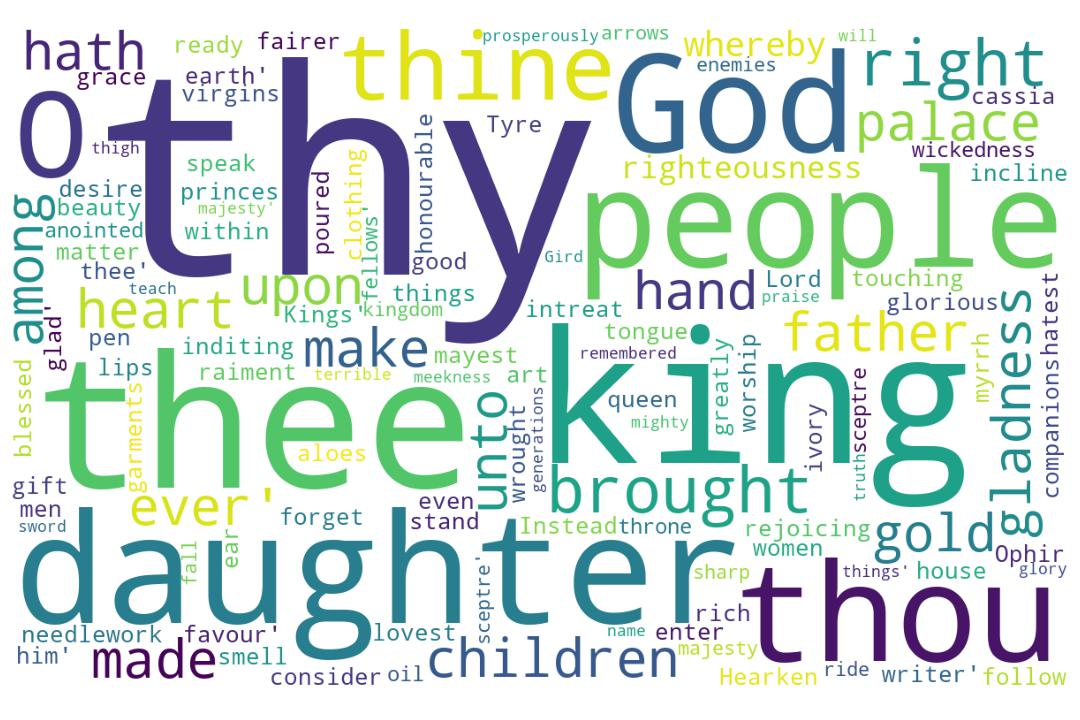
\includegraphics[width=\linewidth]{19OT-Psalms/Psalm45-WordCloud.jpg}
  \caption{Psalm 45 Word Cloud}
  \label{fig:Psalm 45 word Cloud}
\end{figure}

\marginpar{\scriptsize \centering \fcolorbox{bone}{lime}{\textbf{THE WEDDING SCENE}}\\ (Psalm 45:1-17) \begin{compactenum}[I.][8]
    \item A \textbf{Great Husband} \index[scripture]{Psalms!Psa 045:02}(Psa 45:2)
    \item \textbf{Glory \& } \index[scripture]{Psalms!Psa 045:08}(Psa 45:8)
    \item \textbf{Gladness \& Happiness} \index[scripture]{Psalms!Psa 045:07}(Psa 45:7)
    \item The \textbf{Groom is Here} \index[scripture]{Psalms!Psa 045:08}(Psa 45:8)
    \item The \textbf{Guests on High} (one theologian argues -- and I agree -- that the wedding guests will include believers from all ages, such as those before the Law, Gentile believers during the Law, etc -- all there to witness the Lord and His bride)\index[scripture]{Psalms!Psa 045:08}(Psa 45:8)
    \item \textbf{Gifts handed over} \index[scripture]{Psalms!Psa 045:12}(Psa 45:12)
    \item The \textbf{Gown and Handmaidens} \index[scripture]{Psalms!Psa 045:14}(Psa 45:14)
\end{compactenum}}

\footnote{\textcolor[cmyk]{0.99998,1,0,0}{\hyperlink{TOC}{Return to end of Table of Contents.}}}\footnote{\href{https://www.audioverse.org/english/audiobibles/books/ENGKJV/O/Ps/1}{\textcolor[cmyk]{0.99998,1,0,0}{Psalms Audio}}}\textcolor[cmyk]{0.99998,1,0,0}{To the chief Musician upon Shoshannim, for the sons of Korah, Mashil, A Song of loves}\footnote{\textbf{Revelation 19:7-10} - Let us be glad and rejoice, and give honour to him: for the marriage of the Lamb is come, and his wife hath made herself ready. [8] And to her was granted that she should be arrayed in fine linen, clean and white: for the fine linen is the righteousness of saints. [9] And he saith unto me, Write, Blessed are they which are called unto the marriage supper of the Lamb. And he saith unto me, These are the true sayings of God. [10] And I fell at his feet to worship him. And he said unto me, See thou do it not: I am thy fellowservant, and of thy brethren that have the testimony of Jesus: worship God: for the testimony of Jesus is the spirit of prophecy.}\\
\\
\textcolor[cmyk]{0.99998,1,0,0}{My heart is inditing a good matter: I speak of the things which I have made touching the king: my tongue \emph{is} the pen of a ready writer.}
[2] \textcolor[cmyk]{0.99998,1,0,0}{Thou art fairer than the children of men: grace is poured into thy lips: therefore God hath blessed thee for ever.}
[3] \textcolor[cmyk]{0.99998,1,0,0}{Gird thy sword upon \emph{thy} thigh, O \emph{most} mighty, with thy glory and thy majesty.}\footnote{\textbf{Genesis 3:24} - So he drove out the man; and he placed at the east of the garden of Eden Cherubims, and a flaming sword which turned every way, to keep the way of the tree of life.}\footnote{\textbf{Joshua 5:13-15} - And it came to pass, when Joshua was by Jericho, that he lifted up his eyes and looked, and, behold, there stood a man over against him with his sword drawn in his hand: and Joshua went unto him, and said unto him, Art thou for us, or for our adversaries? [14] And he said, Nay; but as captain of the host of the LORD am I now come. And Joshua fell on his face to the earth, and did worship, and said unto him, What saith my lord unto his servant? [15] And the captain of the LORD’S host said unto Joshua, Loose thy shoe from off thy foot; for the place whereon thou standest is holy. And Joshua did so.}\footnote{\textbf{Hebrews 4:12} - For the word of God is quick, and powerful, and sharper than any twoedged sword, piercing even to the dividing asunder of soul and spirit, and of the joints and marrow, and is a discerner of the thoughts and intents of the heart.}\footnote{\textbf{Revelation 19:15} - And out of his mouth goeth a sharp sword, that with it he should smite the nations: and he shall rule them with a rod of iron: and he treadeth the winepress of the fierceness and wrath of Almighty God.}\footnote{\textbf{Revelation 19:21} - And the remnant were slain with the sword of him that sat upon the horse, which sword proceeded out of his mouth: and all the fowls were filled with their flesh.} 
[4] \textcolor[cmyk]{0.99998,1,0,0}{And in thy majesty ride prosperously because of truth and meekness \emph{and} \fcolorbox{bone}{MYGOLD}{righteousness}; and thy right hand shall teach thee terrible things.}
[5] \textcolor[cmyk]{0.99998,1,0,0}{Thine arrows \emph{are} sharp in the heart of the king's enemies; \emph{whereby} the people fall under thee.}
[6] \textcolor[cmyk]{0.99998,1,0,0}{Thy throne, O God, \emph{is} for ever and ever: the sceptre of thy kingdom \emph{is} a right sceptre.}
[7] \textcolor[cmyk]{0.99998,1,0,0}{Thou lovest \fcolorbox{bone}{MYGOLD}{righteousness}, and hatest wickedness: therefore God, thy God, hath anointed thee with the oil of gladness above thy fellows.}
[8] \textcolor[cmyk]{0.99998,1,0,0}{All thy garments \emph{smell} of myrrh, and aloes, \emph{and} cassia, out of the ivory palaces, whereby they have made thee glad.}
[9] \textcolor[cmyk]{0.99998,1,0,0}{Kings' daughters \emph{were} among thy honourable women: upon thy right hand did stand the queen in gold of Ophir.}
[10] \textcolor[cmyk]{0.99998,1,0,0}{Hearken, O daughter, and consider, and incline thine ear; forget also thine own people, and thy father's house;}
[11] \textcolor[cmyk]{0.99998,1,0,0}{So shall the king greatly desire thy beauty: for he \emph{is} thy Lord; and worship thou him.}
[12] \textcolor[cmyk]{0.99998,1,0,0}{And the daughter of Tyre \emph{shall} \emph{be} \emph{there} with a gift; \emph{even} the rich among the people shall intreat thy favour.}
[13] \textcolor[cmyk]{0.99998,1,0,0}{The king's daughter \emph{is} all glorious within: her clothing \emph{is} of wrought gold.}
[14] \textcolor[cmyk]{0.99998,1,0,0}{She shall be brought unto the king in raiment of needlework: the virgins her companions that follow her shall be brought unto thee.}
[15] \textcolor[cmyk]{0.99998,1,0,0}{With gladness and rejoicing shall they be brought: they shall enter into the king's palace.}
[16] \textcolor[cmyk]{0.99998,1,0,0}{Instead of thy fathers shall be thy children, whom thou mayest make princes in all the earth.}
[17] \textcolor[cmyk]{0.99998,1,0,0}{I will make thy name to be remembered in all generations: therefore shall the people praise thee for ever and ever.}




\end{document}

